\documentclass[12pt,letterpaper]{article}

% =============================================================
% TIPOGRAFÍA Y LENGUA
% =============================================================
% El PDF de referencia usa Computer Modern/CM-Super en T1.
% No cargar lmodern, times, newtxtext, libertinus, etc. si se quiere
% conservar la apariencia original.
\usepackage[T1]{fontenc}
\usepackage[utf8]{inputenc}
\usepackage[english]{babel}
\usepackage{indentfirst}

% =============================================================
% GEOMETRÍA: medidas reconstruidas del PDF de referencia
% =============================================================
\usepackage[margin=0.85in]{geometry}
\setlength{\footskip}{20pt}

% =============================================================
% PAQUETES GENERALES
% =============================================================
\usepackage{graphicx}
\usepackage{wrapfig}   % en el preámbulo
\usepackage{amsmath,amssymb,mathtools}
\usepackage{booktabs}
\usepackage{csquotes}
\usepackage{lipsum}
\usepackage{xcolor}
\usepackage[hidelinks]{hyperref}
\usepackage{physics}
\usepackage{amssymb}

%Tablas

\usepackage{multirow}
\usepackage{textcomp}      % Para el símbolo de grado masculino
% =============================================================
% ÍNDICE: reproduce tamaño, espaciado y numeración del PDF
% =============================================================
\usepackage{tocloft}
\renewcommand{\cfttoctitlefont}{\hspace*{226.903bp}\large\bfseries}
\renewcommand{\cftaftertoctitle}{}
\setlength{\cftbeforetoctitleskip}{0pt}
\setlength{\cftaftertoctitleskip}{10pt}
\setcounter{tocdepth}{3}

% =============================================================
% BIBLIOGRAFÍA NUMÉRICA
% =============================================================
\usepackage[
backend=biber, 
style=numeric, 
sorting=none,
maxnames=2, % máximo autores mostrados 
minnames=1, % usa et al. 
giveninits=true, % iniciales en vez de nombres completos 
doi=true, 
url=false, 
isbn=false
]{biblatex} 
\addbibresource{referencias.bib}

% =============================================================
% DATOS EDITABLES DE LA TESIS
% =============================================================
\newcommand{\facultad}{Faculty of Sciences}
\newcommand{\departamento}{Departament of Physics}

% El título del PDF de referencia ocupa dos líneas. Ajusta el salto \\
% manualmente para conservar la composición de la portada.
\newcommand{\titulotesis}{%
Effect of a heterogeneous fitness landscape on 
the threshold for coexistence of phenotypes: 
}
\newcommand{\subtitulotesis}{%
Application to the study of population stability of \textit{Poecilia Reticulata} under predation pressure
}

\newcommand{\autor}{Ángela Valentina Bustos Giraldo}
\newcommand{\correoautor}{av.bustos@uniandes.edu.co}
\newcommand{\asesor}{Juan Manuel Pedraza Leal Ph.D.}
\newcommand{\correoasesor}{jm.pedraza@uniandes.edu.co}
\newcommand{\fechatesis}{\today}


\begin{document}

% ---------- Portada ----------
% =============================================================
% PORTADA
% Posiciones verticales reconstruidas directamente del PDF original.
% =============================================================
\thispagestyle{empty}
\begin{center}

% El logo ocupa exactamente 342.723 bp de ancho en el PDF de referencia.

\includegraphics[width=342.723bp]{figuras/logo_uniandes.png}

\vspace{28.35bp}
{\large\scshape \facultad\\[0pt] \departamento\par}

\vspace{42.5bp}
{\huge\bfseries \titulotesis\par}
{\Large\bfseries \subtitulotesis\par}

\vspace{56.7bp}     
{\bfseries Author:} \autor\\
{\bfseries E-mail:} \correoautor

\vspace{14.2bp}
{\bfseries Advisor:} \asesor\\
{\bfseries E-mail:} \correoasesor

% En el PDF original existe espacio libre para una posible firma del asesor.
% Si se desea añadir una firma como imagen, conviene superponerla y NO
% introducir espacio vertical adicional, para no mover la fecha.

\vfill
{\large Date: \fechatesis}\par
% Ajuste para ubicar la fecha en la misma cota vertical del PDF original.
\vspace*{-9.96bp}

\end{center}

\clearpage

% ---------- Dedicatoria ----------
% =============================================================
% DEDICATORIA
% 12 pt, cursiva, alineada a la derecha y situada en la parte inferior.
% =============================================================
\thispagestyle{empty}
\vspace*{\fill}
\begin{flushright}
\large\itshape
I dedicate this work \\
To all the people who remain in my heart\\
To my mom, my dad, my brother and my grandma\\ 
To my best friend and partner  Álvaro\\
\end{flushright}
% Ajuste inferior obtenido de la posición de la dedicatoria del PDF.
\vspace*{30.67bp}

\clearpage

% En el documento de referencia la página de agradecimientos funciona
% como página lógica 1, aunque el número se oculta. Así el índice queda
% numerado como página 2 y la introducción como página 3.
\setcounter{page}{1}


% ---------- Índice ----------
\tableofcontents
\clearpage

% ---------- Lista de Figuras ----------
\listoffigures
\clearpage


% ---------- Cuerpo ----------
\section{Summary}

This document approaches the dynamics of disadvantageous traits from a biophysical perspective, treating populations as dynamical systems whose evolution is shaped by the interplay between sexual selection, mutation, and predation \cite{nowakEvolutionaryDynamicsExploring2006}. Within this framework, sexual selection is understood as a frequency-dependent process, in which the reproductive value of a trait depends on the traits and choices of other individuals in the population. The aim of this work was to
Develop a stochastic model of phenotype coexistence in a population under sexual selection and predation, based on the Moran process under weak selection, and embed a fitness landscape into the model. The model is instantiated for male guppies (\textit{Poecilia reticulata}), a system chosen because of the extensive empirical data available on sexual selection and predation in this species, which allows the theoretical hypotheses to be tested rather than merely illustrated. 


[Methods]: To this end, we [metodología breve: muestreo, experimento, análisis] muestreo: For these implementations, we used Guppies \textit{Poecilia reticulata} for the extended studies about them, female mate choice strongly favours colourful males \cite{houdeMATECHOICEBASED1987}, yet this same trait increases predation risk \cite{magnhagen1991, godinPredatorPreferenceBrightly2003}. 
 over [periodo o condiciones]. [Results]: Our results show that [hallazgo principal 1] , and that [hallazgo principal 2]. [Conclusion/Implication]: These findings suggest that [interpretación o implicación], providing insight into evolutionary dynamics for sexual selection. 


\begin{center}
    \textit{Keywords: Evolution, Evolutionary Game Theory (EGT), Sexual Selection, Stable Equilibrium States, Noise and Chaos, Moran Process, Poecilia Reticulata}
\end{center}


\clearpage
\section{Introduction}

Interest in understanding how traits change dynamically within populations has driven a substantial body of research examining the role of stochasticity and noise in nature. Every biological population is a system far from equilibrium \footnote{It means that a trait distribution is outside an attractor or at a fixed point, but these systems change due to directional selection, transients, or non-stationary dynamics (such as cycles, stochasticity, or frequency dependence).}, where genetic information and traits flow, interact, and reorganize across time and space. This continuous interplay and variation is what we call evolution. Evolution requires reproduction of information (\cite{lamarckPhilosophieZoologique1809} as discussed in Nowak \cite{nowakEvolutionaryDynamicsExploring2006}), an imperfect process in which error and mutations can occur, these mutations act as a source of stochasticity that perturbs the dynamics of the population  as is discussed in Nowak chapter 2 \cite{nowakEvolutionaryDynamicsExploring2006}. Dynamical systems and stochastic processes offer a framework for thinking about population evolution as a complex system.  In this context, statistical physics provides a formal language for stochasticity and collective change, linking evolutionary dynamics to statistical-style analogies.\footnote{As a curious aside, Barton and Coe \cite{bartonApplicationStatisticalPhysics2009} develop a formal—not literal—analogy between Wright’s stationary allele-frequency distribution and the Boltzmann distribution: population size plays the role of inverse temperature, and log mean fitness that of a negative energy.} In this sense, biophysics is not merely an eclectic combination of disciplines; rather, it is defined by the questions it seeks to answer and its pursuit of general physical principles that transcend the specific details of individual biological systems \cite{bialek2012biophysics}. \\

Yet biology offers numerous cases that challenge this classical expectation. There exist phenotypes that are disadvantageous with predation and/or costly to maintain across generations. Despite this fact, these specific phenotypes persist in the population over generations. Examples include brightness of fireflies \textit{Photinus collustrans}, the long tails of male hummingbirds \textit{Spathura underwoodi}, the scents left by some species of mice \textit{Peromyscus manicultatus bairdi}, and even the chuck sound of certain frogs \textit{Gryllodes integers}\footnote{Refer to the table \ref{tab:1} on the appendix for other examples.}. Each of these species has its specific predator  (\cite{ryan1985,  cushing1985estrous} cited by \cite{magnhagen1991}). This is not consistent with classical evolutionary beliefs, where it is expect that non-adaptive phenotypes would disappear from the population. This can be explained by the deed that these genetic traits are sexually selected, meaning that individuals with these traits have a reproductive advantage, allowing these phenotypes to persist in the population despite associated costs. This data provoked Darwin to develop his theory of sexual selection talked in \cite{andersson1994} (hay que revisar que parte del libro habla de darwin y su teoria de la seleccion natural como tal). \\

A central complication is that the reproductive advantage of a trait often depends on what other individuals among population do. This is the domain of evolutionary game theory \textbf{(EGT)}, which models the fitness of a strategy as a function of its frequency and of the strategies adopted by the rest of the population \cite{nowakEvolutionaryDynamicsExploring2006}. Frequency-dependent interactions can produce stable coexistence of phenotypes, alternative equilibria, or the dominance of a single strategy, none of which can be captured by a fitness that is fixed in advance. Fitness landscapes complement this view, by representing fitness as a function over the space of phenotypes, they provide a geometric intuition for how populations move toward stable points, coexist, or become dominated by a particular phenotype, while also accommodating stochastic phenomena such as mutation inherent to reproduction \cite{bartonApplicationStatisticalPhysics2009}.\\


\subsection{Objetives}
\subsubsection{General Objective}

To develop a theoretical and computational model to investigate the evolution, stability, and coexistence of phenotypes in populations subject to strong sexual selection and predation. The model integrates evolutionary game theory, replicator dynamics, and the stochastic Moran process to characterize evolutionary trajectories through a fitness landscape incorporating demographic noise. The framework is applied to male guppies (\textit{Poecilia reticulata}), using empirical evidence to inform its biological assumptions and parameters.

\subsubsection{Specific Objectives}
\begin{enumerate}
    \item Define the phenotypes, fitness functions, and biological and behavioural hypotheses for the guppy population, and build a payoff matrix that captures the interactions between two phenotypes under different environmental conditions (presence and absence of predation).
    
    \item  Implement the Moran process among sexual selected population as an initial test of the theoretical hypotheses, including a graphical representation of the growth of the preferred sexual trait across successive generations under predation.
    
    \item Determine the conditions that allow for phenotype coexistence, considering the effects of predation and sexual selection.
    
    \item  Explore environmental factors to outline fitness landscapes that can be incorporated into the model, providing a more comprehensive understanding of the dynamics of sexual selection for real populations.
\end{enumerate}


This approach integrates evolutionary game theory, the Moran process under weak selection, and the fitness landscape to investigate the persistence of costly sexual traits \cite{nowakEvolutionaryDynamicsExploring2006,andersson1994}, bridging classical sexual selection models and stochastic dynamics. Applied to guppies (\textit{Poecilia reticulata}), it provides insight into how predation influences phenotype coexistence \cite{houdeMATECHOICEBASED1987,magnhagen1991,houdeSexColorMate1997,endlerNATURALSELECTIONCOLOR1980}, while offering a reproducible framework adaptable to other species. We hypothesize that, under weak selection, two male phenotypes can coexist stably when the reproductive benefits of sexual attractiveness offset predation costs, whereas the preferred phenotype is expected to dominate in the absence of predation.\\


To conclude this section, the document is structured as follows: Chapter 3 presents the theoretical framework, including a review of relevant literature and the development of the model. Chapter 4 describes the methodology used to implement the model and conduct simulations. Chapter 5 presents the results obtained from the simulations and mathematical results, along with an pre-analysis of their implications. Chapter 6 discusses the findings in relation to existing literature and outlines potential avenues for future research. Finally, Chapter 8 provides an appendix with supplementary information and data supporting the study's conclusions.\\
\clearpage
\section{Theoretical Framework}

This framework outlines sexual selection dynamics by combining deterministic and stochastic approaches. We first present Evolutionary Game Theory and stability analysis (Section \ref{sec:EGT} and \ref{sec:SA}) as deterministic foundations, then extend to finite populations using Markov chains, the master equation, and the Fokker--Planck approximation (Sections \ref{sec:Markov}--\ref{sec:fokker}). We discuss the Moran and Wright--Fisher processes as stochastic evolutionary models (Section \ref{sec:Moran}), introduce fitness-landscape parameters to characterize system behavior (Section \ref{sec:fitness}), link these ideas to sexual selection in guppies \textit{Poecilia reticulata} (Section \ref{sec:biology}), and finally examine realistic dynamics via nonlinear parameters (Section \ref{sec:nolinear}).\\ 


\subsection{Evolutionary Game Theory}
\label{sec:EGT}

Evolutionary Game Theory \textbf{(EGT)}, as a branch of game theory\footnote{
Game Theory rose formally in the 20th century. This teory consolidated a fundamental tool  for the analysis of individual strategies in competition contexts, where each individual depends on their actions and the actions of others among their group. Firstly, John von Neumann 1928 had expose about minimax theorem wich talks about of an optimal strategy in the sum of zero game. Then, John von Neumman and Oskar Morgenstern  published in 1944 the book \textit{Theory of Games and Economic Behavior}, which laid the foundations of game theory. Lastly, from 1950 onwards, other authors have been working  in go deeper into this subject as John Nash conceptualized the Nash equilibrium \cite{vonneumann1944, GameTheoryVery, nasar1998}.\\ 
}, initially applied for by John Maynard Smith and George Price  (\cite{maynardsmith1973, maynardsmith1982} explain in Nowak chapter 4  \cite{nowakEvolutionaryDynamicsExploring2006} and \cite{freyEvolutionaryGameTheory2010}). It is a form to simulate natural selection via the interplay between population and their strategies.
It is then a transition from classical rational players to evolutionary forces such as fitness, selection or
mutation. Acording to Frey \cite{freyEvolutionaryGameTheory2010} in a 
jornal as a theorical physics theory, EGT is a mathematical framework that studies the dynamics of
strategic interactions among populations of individuals where  noise have a significant role in the coexistence, evolution, and even extinction of species. In this project, we will focus on well-mixed population \footnote{According to Frey \cite{freyEvolutionaryGameTheory2010} well-mixed describes systems in which individuals move (or diffuse) so extensively that spatial degrees of freedom can be disregarded, and it can be assumed that every individual interacts with all others simultaneously. }.\\

Building on this framework, one can construct a game matrix for purposes of this project, as table \ref{tab:1}, based on two types of phenotypes: those that are sexually selected (A) and those that are not (B), considering predation as a factor of selective pressure. This matrix makes it possible to analyze the interactions between phenotypes and determine the optimal strategies for each. \\ 

\begin{table}[!h]
    \centering
    \begin{tabular}{c|cc}
        & Shoal A& Shoal B\\
        \hline
        Phenotype A & $W_{AA}$ & $W_{AB}$ \\
        Phenotype B & $W_{BA}$ & $W_{BB}$ \\
    \end{tabular}
    \caption{Game matrix for two phenotypes (A (Sexually Selected) and B (Non-Selected)) under sexual selection and predation. The elements $W_{ij}$  represent the payoffs obtained by each phenotype as a function of its interaction with the other.}
    \label{tab:payoffMatrix}
\end{table}



\subsection{Stability Analysis}
\label{sec:SA}
To describe deterministically how the phenotypic composition of the population changes over time, let \(p = \frac{i}{N}\) for a finite population, where \(i\) is the number of individuals of phenotypes \(A\). The dynamics of the frequency of phenotype \(A\) can then be modeled by the continuous-time replicator equation:

\begin{equation}
    \dot{p} = p(1-p)(\Pi_A - \Pi_B)
    \label{eq:p}
\end{equation}


Where 
\begin{equation}
    \Pi_A = p W_{AA} + (1-p) W_{AB}\ \quad  \text{and} \quad \Pi_B = p W_{BA} + (1-p) W_{BB}
    \label{eq:piA}
\end{equation}
\\

Here, \(W_{nm}\) denotes the payoff received by an individual of phenotype \(n\) when interacting with phenotype \(m\). Two additional quantities characterize the evolutionary dynamics are the mean population fitness and the fitness difference between phenotypes, defined respectively as

\begin{equation}
    \overline{\Pi}=p\Pi_A+(1-p)\Pi_B,
    \label{eq:meanPi}
\end{equation}

\begin{equation}
\Delta\Pi=\Pi_A-\Pi_B,
\label{eq:diffPi}
\end{equation}

capture the relative selective advantage of phenotype \(A\) over phenotype \(B\). A positive fitness difference promotes an increase in the frequency of phenotype \(A\), whereas a negative difference favors phenotype \(B\). These quantities therefore provide the basis for identifying evolutionary equilibria and assessing their stability under the replicator dynamics. \\

The equilibria follow from setting \(\dot{p}=0\), and their stability is determined by examining the direction of the evolutionary dynamics near each equilibrium. Depending on the relative fitness values, the system displays four evolutionary regimes in the generic case of strict fitness inequalities, together with the special case of complete neutrality.\\ 

\begin{itemize}
    \item \textbf{A dominates B:} Occurs if \(W_{AA} > W_{BA}\) and \(W_{AB} > W_{BB}\). Phenotype \(A\) always has a higher fitness regardless of the shoal composition, driving the system to the \(p=1\) attractor.\\
  
    \item \textbf{B dominates A:} Occurs if \(W_{AA} < W_{BA}\) and \(W_{AB} < W_{BB}\). The system converges to \(p=0\).\\

    \item \textbf{Bi-stability:} Occurs if \(W_{AA} > W_{BA}\) and \(W_{BB} > W_{AB}\). There are two stable attractors (\(p=0\) and \(p=1\)) separated by an unstable interior equilibrium.\\
    
    \item \textbf{Stable Coexistence:} Occurs if \(W_{AA} < W_{BA}\) and \(W_{BB} < W_{AB}\). The system converges to an interior equilibrium 
    \begin{equation}
        p^* = \frac{W_{BB}-W_{AB}}{W_{AA}-W_{AB}-W_{BA}+W_{BB}}
        \label{eq:pEquilibrium}
    \end{equation}

    where both phenotypes coexist.\\
    
    \item \textbf{Neutrality:} Occurs when \(W_{AA}=W_{BA}\) and \(W_{AB}=W_{BB}\). Both phenotypes have identical fitness for any population composition, resulting in \(\dot{p}=0\) for all \(p\). In finite populations, however, stochastic genetic drift may still produce changes in phenotype frequencies.
\end{itemize}

While the replicator equation characterizes the temporal evolution of phenotype frequencies and the stability of population equilibria, evolutionary stability provides a complementary criterion based on resistance to invasion by rare mutants. This distinction is captured by the concept of an  \textbf{Evolutionarily Stable Strategy (ESS)}, which identifies strategies that cannot be successfully invaded by an initially rare alternative strategy under the assumptions of the evolutionary game according to \cite{mit2021game} and \cite{nowakEvolutionaryDynamicsExploring2006}. For phenotype \(A\) to be an ESS, it must satisfy either:

\begin{itemize}
    \item \textbf{Strict Nash Equilibrium:} \(W_{AA} > W_{BA}\) (A is strictly better than B when playing against A). \\ 
    
    \item \textbf{Weak Nash Equilibrium:} If \(W_{AA} = W_{BA}\), then it must hold that \(W_{AB} > W_{BB}\) (A is better than B when playing against B).
\end{itemize}

\vspace{1em}

\subsection{Markov Chains}
\label{sec:Markov}

 To incorporate the stochastic fluctuations in finite, evolutionary dynamics can be modeled as a discrete-time Markov chain, where changes in population composition are governed by probabilistic transitions between discrete states.

\begin{figure}[h!]
    \centering
    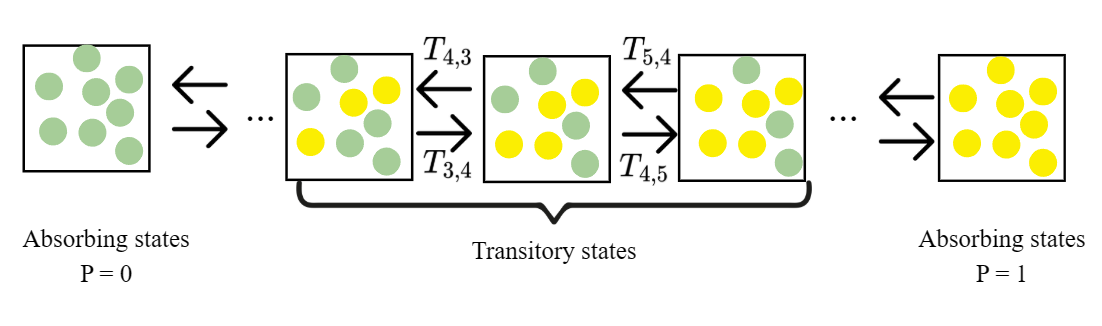
\includegraphics[width=1\linewidth]{Imagenes/Markov Chains.png}
    \caption{Representation of a finite-population Markov chain describing the stochastic evolution of two competing phenotypes A (yellow) and  B (green). Each state represents a population composition, with transitions between neighboring states governed by the probabilities \(T_{i,j}\). The intermediate states are transient, allowing fluctuations in phenotype frequencies, whereas the boundary states \(p=0\) and \(p=1\) are absorbing, corresponding to the fixation of one phenotype and the extinction of the other, inspired by \cite{nowakEvolutionaryDynamicsExploring2006}.}
    \label{fig:markovChains}
\end{figure}    

\clearpage 

Therefore the probability of transitions \(T_{i,j}\) based in the process of Liu et al \cite{liuFixationProbabilitiesEvolutionary2015}, using equations \eqref{eq:piA}, are: 

\begin{equation}
    T_{i,i+1}=  \frac{i \cdot \Pi_A}{i \cdot \Pi_A + (N-i)\cdot \Pi_B}\frac{N-i}{N}
    \label{eq:transicionmas}
\end{equation}

\begin{equation}
    T_{i,i-1}=  \frac{(N-i) \cdot \Pi_B}{i \cdot \Pi_A + (N-i)\cdot \Pi_B}\frac{i}{N}
    \label{eq:transicionmenos}
\end{equation}

\begin{equation}
    T_{i,i}=  1-T_{i,i+1} - T_{i,i-1}
    \label{eq:sintransicion}
\end{equation}

In the absence of mutations, the states \(p=0\) and \(p=1\) are absorbing, corresponding to the extinction and fixation of phenotype \(A\), respectively. The remaining states are transient, allowing stochastic changes in population composition until one of the absorbing states is reached. The process is described in the figure \ref{fig:markovChains}; it is based on birth-death process, specifically in Moran process, it will be described after.\\  

The transition probabilities define a tridiagonal matrix \(M\) of dimensions \((N+1)\times(N+1)\), since the number of individuals exhibiting phenotype A can increase or decrease by at most one during each transition. Each state \(i\in\{0,1,\ldots,N\}\) represents the number of individuals of phenotype A, while the matrix elements \(M_{ij}\) describe the probability of transitioning from state \(i\) to state \(j\). In the absence of mutation, the boundary states \(i=0\) and \(i=N\) are absorbing, corresponding to the fixation of phenotypes B and A, respectively. The transition matrix is therefore expressed as

\begin{equation}
M=
\begin{pmatrix}
1 & 0 & 0 & \cdots & 0 & 0 \\
T_{1,0} & T_{1,1} & T_{1,2} & \cdots & 0 & 0 \\
0 & T_{2,1} & T_{2,2} & \ddots & 0 & 0 \\
\vdots & \ddots & \ddots & \ddots & \ddots & \vdots \\
0 & 0 & \cdots & T_{N-1,N-2} & T_{N-1,N-1} & T_{N-1,N} \\
0 & 0 & \cdots & 0 & 0 & 1
\end{pmatrix}.
\label{eq:moran_transition_matrix}
\end{equation}

For each interior state \(1\leq i\leq N-1\), the transition probabilities satisfy

\begin{equation}
T_{i,i-1}+T_{i,i}+T_{i,i+1}=1.
\end{equation}

The evolution of the population probability distribution is then determined by successive applications of the transition matrix:

\begin{equation}
\mathbf{x}^{(n)}=\mathbf{x}^{(0)}M^n,
\label{eq:markov_evolution}
\end{equation}

where \(\mathbf{x}^{(0)}\) is the initial probability distribution over the population states and \(n\) denotes the number of Markov chain steps.
\clearpage

\subsection{Master Equation}
\label{sec:master}

While the transition probabilities characterize the possible changes in population composition during a single reproduction--replacement event, they do not explicitly describe how the probability distribution over population states evolves over time. This evolution is described by the master equation, which follows from the Markov property and accounts for probability flows between neighboring states. \\ 

Let \(P_i(n)\) denote the probability of finding exactly \(i\) individuals exhibiting phenotype A after \(n\) steps of the Markov chain. For the discrete-time birth--death process considered here, the probability distribution evolves according to

\begin{equation}
    P_i(n+1)
    =
    P_{i-1}(n)T_{i-1,i}
    +
    P_i(n)T_{i,i}
    +
    P_{i+1}(n)T_{i+1,i},
    \label{eq:probDynamics}
\end{equation}

where the three terms represent the probabilities of entering state \(i\) from state \(i-1\), remaining in state \(i\), and entering from state \(i+1\), respectively.\\ 

Equivalently, the master equation can be expressed in terms of the net probability flow between neighboring states:

\begin{equation}
\begin{aligned}
    P_i(n+1)-P_i(n)
    ={}&
    P_{i-1}(n)T_{i-1,i}\\
    &+P_{i+1}(n)T_{i+1,i}\\
    &-P_i(n)\left(T_{i,i+1}+T_{i,i-1}\right).
\end{aligned}
\label{eq:Nose}
\end{equation}

Both expressions apply to the interior states \(1\leq i\leq N-1\). In the absence of mutation, the boundary states \(i=0\) and \(i=N\) are absorbing, corresponding to the fixation of phenotypes B and A, respectively. Their probabilities evolve according to

\begin{equation}
\begin{aligned}
P_0(n+1)&=P_0(n)+P_1(n)T_{1,0},\\
P_N(n+1)&=P_N(n)+P_{N-1}(n)T_{N-1,N}.
\end{aligned}
\label{eq:master_boundaries}
\end{equation}

The master equation can also be written in matrix form as

\begin{equation}
\mathbf{x}^{(n+1)}=\mathbf{x}^{(n)}M,
\label{eq:master_matrix}
\end{equation}

where \(\mathbf{x}^{(n)}\) is the probability distribution over all population states and \(M\) is the transition matrix of the Markov chain. \\ 

This formulation provides a probabilistic description of evolutionary dynamics in finite populations, incorporating both directional selection and demographic fluctuations. Unlike the deterministic replicator equation, it describes the redistribution of probability across population states and allows the temporal evolution of fixation probabilities to be investigated.


\clearpage 


\subsection{Fokker-Planck Continuous Approximation}
\label{sec:fokker}
For sufficiently large populations, a continuous
approximation can be introduced to describe the stochastic
evolution of phenotype frequencies. To obtain this approximation, we define the frequency of
phenotype  \(A\), such that changes between
neighboring states correspond to increments of
\(\Delta p=1/N\). We also introduce the rescaled time
\(\tau=t/N\) and the continuous probability density
\(P(p,\tau)\approx NP_i(t)\). \\ 

Assuming sufficiently smooth transition probabilities
and probability densities, a second-order Kramers--Moyal, as described by Moyal in \cite{moyalStochasticProcessesStatistic1949},
expansion of the master equation yields the
Fokker--Planck approximation: 


\begin{equation}
    \frac{\partial P(p,\tau)}{\partial \tau}
    =
    -\frac{\partial}{\partial p}
    \left[A(p)P(p,\tau)\right]
    +
    \frac{1}{2}
    \frac{\partial^2}{\partial p^2}
    \left[B(p)P(p,\tau)\right].
    \label{eq:FokkerPlanck}
\end{equation}

Here, \(A(p)\) and \(B(p)\) are the drift and diffusion
coefficients, respectively, defined in terms of the
transition probabilities as: 

\begin{equation}
    A(p)=T_{i,i+1}-T_{i,i-1}, \quad   B(p)=\frac{T_{i,i+1}+T_{i,i-1}}{N}, 
    \label{eq:driftCoefficient}
\end{equation}

where the transition probabilities are evaluated at \(i=Np\).Substituting the transition probabilities previouslydefined for the Moran process, the drift coefficient
becomes and the diffusion coefficient is given by, respectively

\begin{equation}
    A(p)=
    \frac{
        p(1-p)(\Pi_A-\Pi_B)
    }{
        p\Pi_A+(1-p)\Pi_B
    }, \quad  B(p)=
    \frac{
        p(1-p)(\Pi_A+\Pi_B)
    }{
        N[p\Pi_A+(1-p)\Pi_B]
    }.
    \label{eq:driftFitness}
\end{equation}

The drift coefficient describes the directional
change in phenotype frequency associated with fitness
differences, while the diffusion coefficient quantifies
the stochastic fluctuations arising from finite
population size.\\ 

In particular, the diffusion coefficient scales
inversely with \(N\), indicating that stochastic
fluctuations become weaker as the population grows.
The resulting Fokker--Planck equation therefore
provides a continuous approximation connecting
stochastic birth--death dynamics with the deterministic
evolutionary framework.


\subsection{Moran Process}
\label{sec:Moran}

This algorithm is a dynamical simulation of a birth-death process (it keeps the population constant), in which an individual from a population is randomly selected to reproduce, with a probability weighted by its fitness. Then, another individual is randomly selected to die and be replaced by the offspring of the first selected individual, as described in figure \ref{fig:moranProcess}. This process is repeated iteratively at each step of the simulation, allowing observation of how the population of a given phenotype spreads or vanishes over time. The probability of fixation of a phenotype depends on its relative fitness and on the composition of the phenotypes, which makes the Moran process a useful tool for studying the evolution of phenotypes under different selective conditions. This process was originally described by Moran \cite{moran1958}, as noted by Galanis et al. \cite{galanisAmplifiersMoranProcess2017} and in Chapter 6 of Nowak \cite{nowakEvolutionaryDynamicsExploring2006}. \\ 


\begin{figure}[h!]
    \centering
    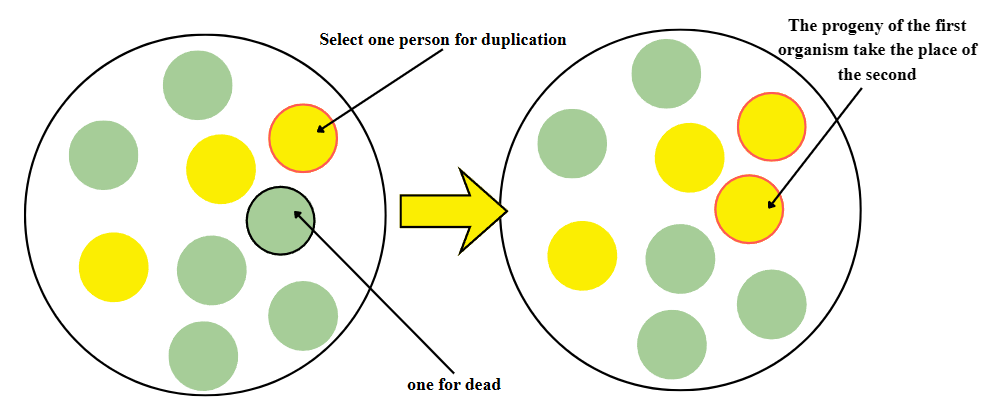
\includegraphics[width=0.9\linewidth]{Imagenes/Moran Process.png}
    \caption{Schematic representation of the Moran process. At each step, in a finite population of $N$ individuals, an individual is selected for reproduction (duplication) with a probability proportional to its fitness (upper arrow), while another is chosen at random to die (lower arrow). The offspring of the first replaces the second, keeping the population size constant. This iterative process allows observation of how phenotypes spread or go extinct over time inspired by \cite{nowakEvolutionaryDynamicsExploring2006}.}
    \label{fig:moranProcess}
\end{figure}


A second type of birth-death process is the Wright–Fisher process, which, like the Moran process, assumes a finite population of constant size \(N\) but differs in its reproductive scheme. In the Wright–Fisher process assumes discrete, non-overlapping generations: all individuals reproduce simultaneously, each contributing offspring to a common pool in proportion to its payoff (fitness), and the next generation is then sampled randomly from this pool—formally, through \(N\). This results in a complete generational turnover at each step, rather than the single-individual replacement of the Moran process 
\cite{imhofEvolutionaryGameDynamics2006}. The Markov chain produced has two absorbing states identical to the original, but given the nearly all differential one-step transitions, it necessitates a different analytical approach. In conclusion, the use of the Moran process is explained by the fact that the Wright–Fisher process would be analytically more complicated than needed for the information the Moran approach provides.  \\ 



\subsection{Fitness Landscape}
\label{sec:fitness}
Originally introduced by Sewall Wright, the fitness landscape visualizes how biological configurations relate to evolutionary fitness; traditionally, it maps fitness across a multidimensional genetic space, revealing peaks, valleys, and regions of differing reproductive success \cite{nowakEvolutionaryDynamicsExploring2006,mccandlishVISUALIZINGFITNESSLANDSCAPES2011}. Here, we adapt this concept to a population of two competing phenotypes, representing the resulting landscape as a three-dimensional surface figure \ref{fig:fitnessLandscape}. Although peaks and valleys denote higher and lower fitness, their correspondence with evolutionary attractors or unstable equilibria must be established through the population dynamics.


\begin{figure}[h!]
    \centering
    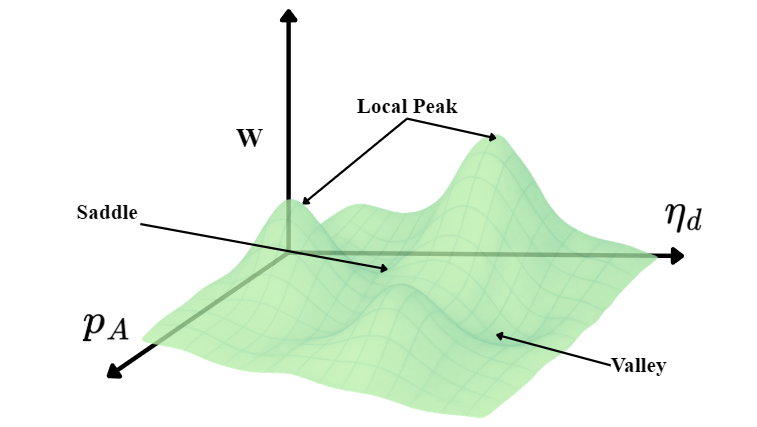
\includegraphics[width=0.75\linewidth]{Imagenes/Fitness Landscape.png}
    \caption{ Three-dimensional fitness landscape showing fitness \(W\)as a function of the initial density of phenotype A \(P_A\) and predator density \(\eta_d\), illustrating key topological features such as local peaks, valleys, and saddle points inspired by \cite{nowakEvolutionaryDynamicsExploring2006} .}
    \label{fig:fitnessLandscape}
\end{figure}

For the two-phenotype system, the fitness landscape can be built from the expected fitness of each phenotype, with the mean population fitness and the fitness difference defined in equations \ref{eq:meanPi} and\ref{eq:diffPi}. Both quantities can be visualized as surfaces, although the fitness difference conveys the direction of selection rather than absolute reproductive success.\\ 


In stochastic simulations, the mean change over a finite interval of \(x\) Moran steps can be estimated by averaging the slopes of \(R\) independent trajectories initialized at the same population composition:

\begin{equation}
\widehat{v}_x(p_0,\eta_d)
=
\frac{1}{R}
\sum_{r=1}^{R}
\frac{p_r(x)-p_0}{x},
\end{equation}

where \(p_r(x)\) is the proportion of phenotype \(A\) after \(x\) steps in realization \(r\). Evaluating this quantity across initial frequencies \(p_0\) and predation intensities \(\eta_d\) yields a three-dimensional surface representing a finite-time drift landscape, which characterizes the direction and magnitude of the mean evolutionary change. \\ 

From a physical perspective, evolutionary drift provides a useful analogy with a force field, as it describes the expected direction and magnitude of changes in population composition. In a one-dimensional evolutionary state space, an effective potential can be formally constructed by integrating the negative instantaneous drift with respect to the phenotypic frequency. However, this potential must be distinguished from mean population fitness, whose gradient does not generally determine the evolutionary dynamics. Furthermore, the drift field alone does not fully characterize stochastic evolution, since demographic fluctuations also contribute to the redistribution of probability across population states. This distinction motivates the complementary use of fitness landscapes, evolutionary drift, and stochastic population models.\\ 

\clearpage


\subsection{Biological Dynamics for Sexual Selection Poblation}
\label{sec:biology}

\begin{wrapfigure}{l}{0.5\textwidth}
    \centering
    \vspace{-1em}
    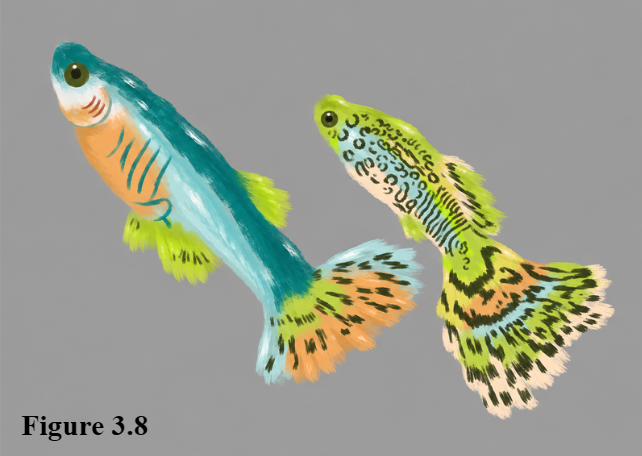
\includegraphics[width=\linewidth]{Imagenes/Guppies.png}
    \label{fig:guppiesdisform}
    \vspace{-2em}
\end{wrapfigure}

Although the theoretical framework developed in this study does not require a specific biological species, male guppies (\textit{Poecilia reticulata}) provide a suitable reference system due to the extensive experimental literature on sexual selection and predation. Guppies exhibit pronounced sexual dimorphism, with males displaying more conspicuous colour patterns than females, as illustrated in Figure \ref{fig:guppiesdisform}. Male reproductive success is strongly influenced by female mate choice and sexual attractiveness, consistent with the theory of secondary sexual traits \cite{andersson1994,houdeSexColorMate1997}. In particular, Houde \cite{houdeMATECHOICEBASED1987} demonstrated that female guppies preferentially associate and mate with males exhibiting larger areas of orange pigmentation, while Zahavi's handicap principle suggests that costly ornamentation may serve as a signal of individual quality \cite{zahavi1987signal}. However, these sexually attractive traits may also increase vulnerability to predators, generating opposing selective pressures. Godin and McDonough \cite{godinPredatorPreferenceBrightly2003} experimentally demonstrated that predatory cichlids preferentially attacked and captured more brightly coloured males, while female mating preferences and male reproductive behaviour may change in response to predation risk \cite{godinFemaleMateChoice1996,magnhagen1991}. Furthermore, the effectiveness and survival costs of visual signals depend on environmental conditions and their perception by potential mates and predators \cite{endler1991}. Predation pressure may also influence courtship displays, alternative mating tactics, and reproductive risk-taking behaviour \cite{bothamRISKSENSITIVEANTIPREDATORBEHAVIOR2008,smithBehavioralTypesPredictors2010,goslinePredatorinducedPlasticityGuppy2008}. Endler \cite{endlerNATURALSELECTIONCOLOR1980} demonstrated that predation regimes can shape the evolution of male coloration, with reduced predation generally favouring greater ornamentation and stronger predation favouring less conspicuous phenotypes. These observations illustrate the trade-off between reproductive attractiveness and predation-related survival costs, making guppies a biologically motivated reference system for investigating the evolutionary dynamics of alternative male phenotypes.\\ 

From a biological perspective, frequency dependence may arise from changes in predation vulnerability associated with the phenotypic composition of a shoal. Conspicuous individuals exhibit highly visible traits, such as bright coloration, whereas cryptic individuals display traits that reduce their detectability against the surrounding environment. Consequently, predominantly conspicuous groups may attract greater predator attention than cryptic groups. However, individual predation risk also depends on group composition: the \textit{oddity effect} may increase the vulnerability of individuals whose appearance differs from that of other group members, while the \textit{confusion effect} may reduce a predator's ability to identify and capture a particular individual within a group \cite{rodgersMixedphenotypeGroupingInteraction2013}. Although these mechanisms may operate asymmetrically, their opposing contributions are assumed to approximately compensate under the reference conditions considered, without implying universal cancellation. These biological mechanisms suggest that the fitness of each phenotype may depend not only on predation intensity and reproductive advantages, but also on the phenotypic composition of the population. This motivates the introduction of frequency-dependent
interactions in the evolutionary game-theoretic model.\\ 


\subsection{Nonlinear Parameters in Evolutionary Game Theory}
\label{sec:nolinear}

In classical evolutionary game theory \textbf{(EGT)}, payoff matrices generally contain constant entries, leading to expected fitness functions that depend linearly on population frequencies. However, this approximation may be insufficient for ecological systems in which the costs and benefits of interactions vary with population composition or the frequency of competing phenotypes. More general formulations allow the payoff matrix itself to depend on the evolutionary state of the population, introducing additional nonlinearities into the fitness functions \cite{broomNonlinearMultiplayerEvolutionary2016}. In this case, the payoff matrix becomes frequency-dependent, \(W=W(p)\), and the expected fitness functions are expressed as 

\begin{equation}
\begin{aligned}
\Pi_A(p) &= pW_{AA}(p)+(1-p)W_{AB}(p),\\
\Pi_B(p) &= pW_{BA}(p)+(1-p)W_{BB}(p).
\end{aligned}
\end{equation}

Consequently, the fitness difference \(\Delta\Pi(p)=\Pi_A(p)-\Pi_B(p)\) is generally nonlinear. Although the replicator equation retains its original structure,

\begin{equation}
\dot p=p(1-p)\Delta\Pi(p),
\end{equation}

the location and stability of evolutionary equilibria may change. The boundary equilibria \(p=0\) and \(p=1\) remain stationary, whereas interior equilibria satisfy \(\Delta\Pi(p^*)=0\)  , with \(0<p^*<1\). Their local stability is determined by

\begin{equation}
\left.\frac{d\dot p}{dp}\right|_{p=p^*}
=
p^*(1-p^*)
\left.\frac{d\Delta\Pi}{dp}\right|_{p=p^*}.
\label{eq:estabilidad}
\end{equation}

Thus, a negative derivative of the fitness difference indicates local asymptotic stability, while a positive derivative indicates instability. Similarly, \(p=0\) is locally asymptotically stable when \(\Delta\Pi(0)<0\), and \(p=1\) is locally asymptotically stable when \(\Delta\Pi(1)>0\). Equality cases require further analysis. Importantly, the mathematical frameworks of Markov chains, the master equation, and the Fokker--Planck approximation remain applicable without changes to their general structure. However, the transition probabilities and the corresponding drift and diffusion coefficients must be evaluated using the frequency-dependent fitness functions. \\ 



\clearpage

\section{Methodology}
\label{sec:methodology}

To construct and characterize evolutionary landscapes, three models of increasing complexity were considered: first, a constant-payoff model; second, a frequency-dependent payoff model; and finally, a nonlinear extension incorporating an additional reproductive contribution.
These models describe the interplay between sexual selection and predation in male guppies \textit{Poecilia Reticulata}, providing a biological framework for examining how different fitness formulations influence evolutionary tendencies. Deterministic stability analysis and replicator dynamics were employed to identify the equilibrium structure of each model, while the Moran process, Markov chains, and the master equation were used to incorporate stochastic evolutionary effects. Together, these approaches provided the basis for constructing and comparing mean-fitness, fitness-difference, and evolutionary drift surfaces. Numerical calculations were performed in Python using \texttt{NumPy} and \texttt{SciPy}, while \texttt{Matplotlib} and \texttt{Plotly} were employed for visualization. \\ 



\subsection{Biological Parameters}
\label{sec:biological_parameters}

The evolutionary models incorporate biologically motivated parameters representing sexual selection, predation vulnerability, and genetic variation in male guppies. The parameters $S_a$ and $S_b$ characterize the relative reproductive success of phenotypes A and B, respectively, while $D_a$ and $D_b$ represent their corresponding predation-related penalties. These contributions are introduced as modifications to a common baseline fitness. The sexual selection parameters ($S_a=0.86$, $S_b=0.53$), whereas the predation parameters ($D_a=0.107$, $D_b=0.023$). The relative differences between the corresponding model factors were calculated as

\begin{equation}
    \left(\frac{1+S_a}{1+S_b}-1\right)\times100
    \approx 21.57\%,
    \label{eq:relativeSucess}
\end{equation}

and

\begin{equation}
    \left(\frac{1+D_a}{1+D_b}-1\right)\times100
    \approx 8.21\%.
    \label{eq:relativeDead}
\end{equation}

For the optional mutation mechanisms, the characteristic mutation-related timescale was estimated as $\mu^*\approx1.42\times10^3$ generations, corresponding to the mean waiting time for a mutation within one copy of the genomic region considered. This value provides a reference for the mutation schemes incorporated into the stochastic simulations, rather than a directly measured rate of phenotypic change. The estimation procedures and underlying biological assumptions are detailed in Appendix \ref{sec: Appendix Sa, Sb, Da, Db, mutation}.\\

The evolutionary state is represented by the frequency $p\in[0,1]$ of phenotype A, while $1-p$ represents the frequency of phenotype B. Predation intensity is described by the dimensionless parameter $\eta_d\in[0,1]$. These variables define the parameter space used to construct the evolutionary landscapes. Additional parameters are introduced in the corresponding models. In particular, $r_0$ controls an additional reproductive advantage, whereas $\eta_c$ defines a characteristic predation threshold in the nonlinear extension. The baseline biological parameters were held fixed across the three model formulations to isolate the effects of their different mathematical structures on the resulting evolutionary landscapes. 


\subsection{Constant-Payoff Model}
\label{sec:constant_payoff_methodology}

The first model was formulated using a payoff matrix whose entries are independent of phenotypic frequency. This approximation provides a baseline evolutionary landscape in which reproductive and predation-related contributions depend on environmental conditions but not directly on population composition. The entries of the payoff matrix were defined as

\begin{equation}
W_{AA}(\eta_d)=\frac{1+S_a(1-\eta_d)}{1+D_a\eta_d},
\qquad
W_{AB}(\eta_d,r_0)=W_{AA}(\eta_d)+r_0.
\label{eq:constant_payoff_A}
\end{equation}

\begin{equation}
W_{BA}(\eta_d)=\frac{1+S_b(1-\eta_d)}{1+D_b\eta_d},
\qquad
W_{BB}(\eta_d)=W_{BA}(\eta_d).
\label{eq:constant_payoff_B}
\end{equation}

The parameter $r_0\in[0,0.25]$ represents an additional reproductive advantage of phenotype A when interacting with phenotype B. The resulting expected fitness functions are

\begin{equation}
\Pi_A(p,\eta_d,r_0)=W_{AA}(\eta_d)+(1-p)r_0.
\label{eq:constant_fitness_A}
\end{equation}

\begin{equation}
\Pi_B(p,\eta_d)=W_{BB}(\eta_d).
\label{eq:constant_fitness_B}
\end{equation}


Although the payoff entries do not depend explicitly on \(p\), the expected fitness of phenotype A varies linearly with its frequency through the relative abundance of phenotype B. The model therefore provides a simple analytical reference for examining how the additional reproductive advantage modifies the fitness difference across population compositions. In particular,

\begin{equation}
\Delta\Pi(p,\eta_d,r_0)
=
W_{AA}(\eta_d)-W_{BB}(\eta_d)
+r_0(1-p).
\label{eq:constant_fitness_difference}
\end{equation}

The equilibrium structure associated with this expression was investigated using the stability conditions of evolutionary game theory. Representative parameter combinations were identified through numerical optimization and root-finding routines implemented in \texttt{SciPy}. In addition, a systematic sweep was performed over values of \(\eta_d\in[0,1]\) and values of \(r_0\in[0,0.25]\) to classify the resulting evolutionary regimes. \\ 


\subsection{Frequency-Dependent Payoff Model}
\label{sec:frequency_dependent_methodology}

The second model introduces an explicit dependence of the payoff entries on phenotypic frequency. This extension was developed to examine how population composition modifies the selective advantages of the competing phenotypes and, consequently, the structure of the corresponding evolutionary landscapes. \footnote{The additional reproductive parameter \(r_0\) was omitted in this formulation to isolate the effects of frequency-dependent payoffs.} The payoff entries were defined as


\begin{equation}
W_{AA}(\eta_d)=\frac{1+S_a(1-\eta_d)}{1+D_a\eta_d},
\qquad
W_{AB}(p,\eta_d)=\frac{1+S_a(1-\eta_d)}{1+D_a\eta_d p}.
\label{eq:frequency_dependent_A}
\end{equation}

\begin{equation}
W_{BA}(p,\eta_d)=\frac{1+S_b(1-\eta_d)}{1+D_b\eta_d(1-p)},
\qquad
W_{BB}(\eta_d)=\frac{1+S_b(1-\eta_d)}{1+D_b\eta_d}.
\label{eq:frequency_dependent_B}
\end{equation}

The frequency-dependent denominators introduce different predation-related contributions according to the relative abundance of phenotypes A and B. The expected fitness functions are consequently given by

\begin{equation}
\Pi_A(p,\eta_d)
=
pW_{AA}(\eta_d)
+(1-p)W_{AB}(p,\eta_d).
\label{eq:frequency_fitness_A}
\end{equation}

\begin{equation}
\Pi_B(p,\eta_d)
=
pW_{BA}(p,\eta_d)
+(1-p)W_{BB}(\eta_d).
\label{eq:frequency_fitness_B}
\end{equation}

Unlike the constant-payoff model, the frequency dependence of the payoff entries introduces a nonlinear relationship between phenotypic composition and expected fitness. Consequently, the fitness difference $\Delta\Pi(p,\eta_d)$ may exhibit multiple zeros and changes in sign, potentially giving rise to different equilibrium configurations and stability regimes. These features were investigated numerically by identifying equilibrium solutions and evaluating their stability using the complete frequency-dependent fitness functions. A systematic sweep over $\eta_d\in[0,1]$ was performed to examine how predation intensity modifies the equilibrium structure and the direction of evolutionary selection. \\ 


\subsection{Nonlinear Reproductive-Advantage Model}
\label{sec:nonlinear_reproductive_methodology}

The third model extends the frequency-dependent formulation by introducing a nonlinear reproductive contribution that depends simultaneously on phenotypic frequency and predation intensity. The purpose of this extension is to investigate how an additional ecological constraint on reproductive success modifies the resulting evolutionary landscape.  The nonlinear contribution was defined as

\begin{equation}
r(p,\eta_d,\eta_c,r_0)
=
S_a r_0(1-p)
\max\left(0,1-\frac{\eta_d}{\eta_c}\right),
\label{eq:nonlinear_reproductive_term}
\end{equation}

where \(r_0\) determines the magnitude of the additional reproductive contribution and \(\eta_c\) represents a characteristic predation threshold.  The factor \(1-p\) introduces a decreasing contribution as phenotype A becomes more abundant, while the predation-dependent factor progressively suppresses the additional advantage as \(\eta_d\) approaches \(\eta_c\). For \(\eta_d\geq\eta_c\), the nonlinear contribution vanishes. \\ 

In the current computational formulation, this term was incorporated into the payoff \(W_{AA}\):

\begin{equation}
W_{AA}^{(3)}(p,\eta_d)
=
\frac{1+S_a(1-\eta_d)}{1+D_a\eta_d}
+
r(p,\eta_d,\eta_c,r_0).
\label{eq:nonlinear_WAA}
\end{equation}


The equilibrium structure of the constant-payoff model was examined using evolutionary stability conditions, numerical root-finding, and parameter optimization implemented in \texttt{SciPy}. A systematic exploration of the parameter space $(\eta_d,r_0)$ was performed to classify the evolutionary regimes and identify representative parameter combinations. The deterministic behavior was visualized through replicator trajectories and evolutionary flow diagrams, allowing equilibrium stability and the direction of selection to be examined. The corresponding fitness difference and mean population fitness were represented as three-dimensional surfaces over phenotypic frequency and predation intensity. Stochastic analyses based on the Moran process were also used to examine fixation probabilities, population-frequency trajectories, and evolutionary drift. These representations establish a baseline for comparing the effects of the additional mechanisms introduced in the subsequent models.  \\ 


The three models were subsequently examined using a common deterministic and stochastic framework. Equilibrium configurations and their stability were characterized through evolutionary game theory, while the replicator equation was integrated numerically to study evolutionary trajectories under different initial conditions. Stochastic dynamics were investigated using the Moran process, Markov chains, and the master equation to analyze phenotypic fluctuations, fixation probabilities, and absorption times. These simulations were complemented by evolutionary flow diagrams and heatmaps illustrating changes in population composition across predation intensities. Finally, mean-fitness, fitness-difference, and evolutionary drift landscapes were constructed or estimated, as applicable, to characterize and compare the selective tendencies associated with each model.\\ 


\subsection{Stochastic Evolutionary Drift from the Moran Process}
\label{sec:moran_methodology}

To incorporate demographic fluctuations into the evolutionary landscape, a finite-population Moran process was implemented for each payoff model. The population was represented by \(N\) individuals belonging to one of two phenotypic classes, with its state determined by the number \(i\) of individuals exhibiting phenotype A. \\ 

At each step of the process, one individual was selected for reproduction with a probability proportional to its expected fitness, while another individual was selected uniformly for replacement. Consequently, the frequency of phenotype A could increase by \(1/N\), decrease by \(1/N\), or remain unchanged. \\ 

The probabilities of these events were calculated using the expected fitness functions of the corresponding model:

\begin{equation}
T_i^+
=
\frac{i\Pi_A}{i\Pi_A+(N-i)\Pi_B}
\frac{N-i}{N},
\label{eq:method_moran_plus}
\end{equation}

\begin{equation}
T_i^-
=
\frac{(N-i)\Pi_B}{i\Pi_A+(N-i)\Pi_B}
\frac{i}{N}.
\label{eq:method_moran_minus}
\end{equation}

The probability of remaining in the same state was obtained from \(T_i^0=1-T_i^+-T_i^-\). \\ 

These probabilities define the expected change in phenotypic frequency during a single reproduction--replacement event. The corresponding evolutionary drift is

\begin{equation}
v_M(p,\eta_d)
=
\frac{T_i^+-T_i^-}{N},
\label{eq:method_moran_drift}
\end{equation}

where \(p=i/N\). Substituting the transition probabilities yields

\begin{equation}
v_M(p,\eta_d)
=
\frac{p(1-p)}{N}
\frac{\Pi_A(p,\eta_d)-\Pi_B(p,\eta_d)}
{\overline{\Pi}(p,\eta_d)},
\label{eq:method_moran_drift_fitness}
\end{equation}

with \(\overline{\Pi}=p\Pi_A+(1-p)\Pi_B\). \\ 

This expression provides a direct connection between the payoff-based evolutionary model and the expected stochastic change in population composition. Since the expected fitness values are positive, the sign of the drift in interior states is determined by the fitness difference. Its magnitude, however, also depends on population size, population composition, and mean fitness. \\ 

Individual realizations of the Moran process were generated to examine fluctuations around this expected behavior. The expected fitness values were recalculated after each change in population composition, preserving the frequency dependence of the corresponding payoff model. \\ 

The main computational framework considered population sizes \(N=10\) and \(N=100\), with stochastic trajectories of up to \(10^4\) reproduction--replacement events. The simulations were performed without mutation for the principal landscape calculations, so that the states \(p=0\) and \(p=1\) remained absorbing. \\ 

The principal role of these simulations was to obtain and evaluate the evolutionary drift associated with the different fitness formulations, rather than to reconstruct individual biological population histories. \\ 


\subsection{Markov Chains and Master Equation}
\label{sec:markov_methodology}

The finite-population Moran process was represented as a discrete-time Markov chain with \(N+1\) possible states, corresponding to \(i=0,1,\ldots,N\) individuals exhibiting phenotype A. The transition probabilities obtained from the expected fitness functions were assembled into a tridiagonal transition matrix \(M\), whose nonzero entries describe transitions between neighboring population states and the probability of remaining in the same state. \\ 

In the absence of mutation, the boundary states \(i=0\) and \(i=N\) were defined as absorbing. The initial probability distribution was concentrated at the state corresponding to approximately equal proportions of the two phenotypes:

\begin{equation}
x_i^{(0)}
=
\begin{cases}
1, & i=\lfloor N/2\rfloor,\\
0, & \text{otherwise}.
\end{cases}
\label{eq:initial_markov_distribution}
\end{equation}

The probability distribution was evolved through successive applications of the transition matrix,

\begin{equation}
\mathbf{x}^{(n+1)}
=
\mathbf{x}^{(n)}M,
\label{eq:method_markov_evolution}
\end{equation}

where \(n\) represents the number of Markov chain steps. This numerical implementation corresponds to the discrete master equation introduced in the theoretical framework. \\ 

The cumulative fixation probabilities of phenotypes A and B were obtained from the boundary components \(x_N^{(n)}\) and \(x_0^{(n)}\), respectively. The probability of remaining in transient population states was calculated as 

\begin{equation}
P_{\mathrm{transient}}(n)
=
\sum_{i=1}^{N-1}x_i^{(n)}.
\label{eq:method_transient_probability}
\end{equation}

The temporal mean and variance of the phenotype frequency were also evaluated from the evolving probability distribution. These quantities allow the expected population composition and its fluctuations to be examined without relying exclusively on individual stochastic trajectories. \\

To characterize the persistence of transient states, the mean absorption time was calculated using the transient submatrix \(Q\), obtained by removing the absorbing states from \(M\). The vector of mean absorption times was determined by solving

\begin{equation}
(I-Q)\mathbf{t}=\mathbf{1}.
\label{eq:method_mean_absorption}
\end{equation}

Eventual fixation probabilities were similarly obtained by solving the corresponding linear system for absorption into the phenotype-A boundary state. \\ 

A separate numerical convergence criterion was defined as the first Markov chain step for which the total transient probability became smaller than a prescribed tolerance \(\varepsilon\). In the main parameter sweeps, \(\varepsilon=10^{-6}\) was used, with a maximum of \(10^5\) iterations for the convergence test. The evolution of the probability distribution was additionally evaluated over \(15\,000\) steps. \\ 

These calculations provide a probabilistic reference for interpreting the evolutionary landscapes. In particular, they allow the expected local direction of evolution to be distinguished from the long-term effects of stochastic absorption, which may occur even when the deterministic model possesses a stable interior equilibrium.

\subsection{Construction of Evolutionary Fitness Landscapes}
\label{sec:fitness_methodology}

The central computational procedure of this investigation consists of constructing evolutionary surfaces that characterize the dependence of fitness and evolutionary change on population composition and environmental conditions.

For each evolutionary model, the expected fitness functions were evaluated as functions of phenotype-A frequency \(p\) and predation intensity \(\eta_d\). These variables define a two-dimensional parameter space over which three complementary quantities can be represented: mean population fitness, the fitness difference between phenotypes, and evolutionary drift.

The mean population fitness was calculated as

\begin{equation}
\overline{\Pi}(p,\eta_d)
=
p\Pi_A(p,\eta_d)
+
(1-p)\Pi_B(p,\eta_d).
\label{eq:method_fitness_landscape}
\end{equation}

This quantity describes the average expected reproductive performance of the population at a given phenotypic composition and predation intensity. Its surface representation allows regions of comparatively high and low population fitness to be identified.

The relative selective advantage between phenotypes was characterized through the fitness difference,

\begin{equation}
\Delta\Pi(p,\eta_d)
=
\Pi_A(p,\eta_d)-\Pi_B(p,\eta_d).
\label{eq:method_fitness_difference}
\end{equation}

Positive values of \(\Delta\Pi\) indicate a selective advantage for phenotype A, whereas negative values indicate an advantage for phenotype B. The condition \(\Delta\Pi=0\) identifies compositions where neither phenotype has a relative fitness advantage, providing a direct connection between the fitness-difference surface and the equilibrium structure obtained from the replicator equation.

Unlike the mean-fitness surface, the fitness-difference surface therefore contains explicit directional information about selection. However, it does not by itself describe the rate of stochastic evolutionary change, which also depends on population size and the normalization of reproductive probabilities.

To characterize this directional behavior in finite populations, the evolutionary drift was considered as a third surface,

\begin{equation}
Z_v(p,\eta_d;N)
=
v_M(p,\eta_d;N),
\label{eq:method_drift_surface}
\end{equation}

where \(v_M\) is the expected change in phenotype-A frequency per Moran step.

The three quantities were evaluated numerically over grids of phenotype frequencies and predation intensities. The resulting values were organized as matrices representing surfaces in a three-dimensional coordinate system, with \(p\) and \(\eta_d\) defining the horizontal coordinates and the corresponding evolutionary quantity defining the vertical coordinate.

The constant-payoff model was used to implement and evaluate the initial surface-construction procedures. The same framework was designed to accommodate the frequency-dependent and nonlinear payoff functions, enabling a systematic comparison of landscape structures as the biological complexity of the model increases.

The surfaces were treated as complementary representations rather than interchangeable definitions of a single evolutionary potential. In particular, high mean fitness does not necessarily imply an evolutionarily stable population composition, while the sign of the fitness difference and the evolutionary drift directly indicates the local direction of evolutionary change.

\subsection{Numerical Estimation of the Evolutionary Drift Landscape}
\label{sec:stochastic_drift_methodology}

In addition to the analytical expression for the expected Moran drift, a numerical estimator was constructed from independent stochastic population trajectories. This procedure was designed to characterize the average evolutionary displacement generated by selection and demographic fluctuations over a finite number of reproduction--replacement events. \\ 

For a prescribed initial phenotype frequency \(p_0\) and predation intensity \(\eta_d\), \(R\) independent realizations of the Moran process were simulated. Each realization was evolved for \(k\) Markov chain steps, and the change in phenotype-A frequency was recorded. \\ 

The mean evolutionary drift over the selected interval was estimated as

\begin{equation}
\widehat{v}_k(p_0,\eta_d)
=
\frac{1}{R}
\sum_{r=1}^{R}
\frac{p_r(k)-p_r(0)}{k},
\label{eq:method_empirical_drift}
\end{equation}

where \(p_r(0)\) and \(p_r(k)\) denote the initial and final frequencies in realization \(r\). \\ 

This estimator measures the average finite-time change in phenotypic frequency per Markov chain step. Unlike the instantaneous drift calculated directly from the transition probabilities, the estimator incorporates changes in the population state throughout the simulation interval.\\ 

For each parameter combination, the sample standard deviation of the individual frequency-change rates was calculated, together with the corresponding standard error,

\begin{equation}
\operatorname{SE}(\widehat v_k)
=
\frac{s_v}{\sqrt{R}},
\label{eq:method_drift_error}
\end{equation}

where \(s_v\) is the sample standard deviation of the rates obtained from the independent realizations. \\ 

The estimator was evaluated over a grid of initial frequencies and predation intensities. Each grid point was associated with a separate group of stochastic realizations, and the resulting average rates were assembled into a three-dimensional evolutionary drift surface,

\begin{equation}
Z_{\mathrm{drift}}(p_0,\eta_d)
=
\widehat v_k(p_0,\eta_d).
\label{eq:method_empirical_drift_surface}
\end{equation}

The initial numerical implementation considered population sizes \(N=10\) and \(N=100\), using ten values of the initial phenotype frequency and ten values of predation intensity. For the constant-payoff model, five reproductive-advantage values were examined over \(r_0\in[0,0.25]\). Each surface point was estimated using five independent realizations of \(10^4\) Moran steps. \\

The resulting landscape describes the average displacement of the evolutionary state over the prescribed observation interval. Positive values indicate a net tendency toward increasing phenotype-A frequency, while negative values indicate a net tendency toward decreasing frequency. \\ 

Because the estimator is based on finite-time displacements, its numerical values may depend on the duration of the simulation, population size, and initial condition. It was therefore distinguished from the instantaneous Moran drift, even though both quantities describe directional evolutionary change. \\ 

This stochastic construction provides the principal numerical tool for investigating how the evolutionary landscape is modified by population size, predation intensity, and the mathematical form of the fitness functions.


\subsection{Gaussian Smoothing and Surface Visualization}
\label{sec:landscape_visualization}

The stochastic drift surfaces obtained from a finite number of realizations exhibit fluctuations associated with sampling variability. To facilitate visualization of their large-scale structure, a two-dimensional Gaussian filter was applied to the estimated mean-drift values. \\ 

The smoothing procedure was implemented using \texttt{scipy.ndimage.gaussian\_filter}, with a standard deviation of \(\sigma=1\) in grid units. The filter was applied after averaging the independent stochastic realizations, rather than directly to the individual trajectories. \\ 

For the mutation-free simulations, the drift values at the absorbing boundaries \(p_0=0\) and \(p_0=1\) were preserved after filtering. This prevents the smoothing operation from introducing artificial evolutionary changes at population compositions where the original stochastic process is absorbing. \\ 

Both the unfiltered and Gaussian-smoothed surfaces were retained for comparison. The unfiltered estimates were used as the quantitative reference, while the smoothed representations were employed to improve the visual identification of broad directional patterns. \\ 

The mean-fitness, fitness-difference, and evolutionary drift surfaces were represented using three-dimensional graphical routines implemented in Plotly. The corresponding parameter values and population sizes were included in the visualizations to allow comparisons between different evolutionary conditions. \\ 

Smoothing was treated exclusively as a visualization procedure. In particular, changes in the apparent location of zero crossings, extrema, or equilibrium boundaries introduced by filtering were not considered sufficient evidence of changes in the underlying evolutionary system. \\ 
\clearpage
\section{Results}

Porta eget eu magnis luctus vestibulum ad interdum litora platea neque sed at felis urna velit, a fusce laoreet aptent sapien fringilla montes posuere facilisi iaculis orci libero penatibus nullam. Montes scelerisque quisque phasellus praesent per sed iaculis, porttitor proin penatibus varius luctus cras primis cubilia, fusce rhoncus vestibulum magnis vitae tincidunt. Dignissim mollis lacus pharetra semper lobortis id convallis natoque porta orci, magnis venenatis sodales erat metus integer vitae habitasse conubia, congue est enim dis interdum quisque egestas sociosqu aenean \footnote{ I prefer not to show all my attempts in this document but I have made a previous analysis and documentation
on a Jupyter Notebook that can be found at \url{https://github.com/ValentinaBustos2025/Proyecto-Final} in a Jupyter Notebook, in the file
\textbf{Simulación/Simulacion Principal.ipynb}.}. \\


\subsection{Constant-Payoff Evolutionary Regimes}



As mentioned in the methodology, the python \texttt{scipy.optimize} library was used to find the values of  \(\eta_d\)  and  \(r_0\)  giving summarized values in the table \ref{tab:linermatrixdynamics}.  To illustrate these regimes, figure \ref{fig:replicator} presents the evolutionary trajectories of the proportion of phenotype A, \(p(t)\), for representative combinations of \(\eta_d\) and \(r_0\), considering different initial population compositions. The boundary conditions \(p=0\), corresponding to a population composed entirely of phenotype B, and \(p=1\), corresponding to a population composed entirely of phenotype A, were excluded from the plotted initial conditions because both are stationary states of the replicator equation (\(\dot{p}=0\)), where the phenotypic composition remains unchanged. Therefore, only initial frequencies satisfying \(0<p(0)<1\) were considered to visualize the evolution of the population toward the corresponding equilibria. 

\begin{figure}[h!]
    \centering
    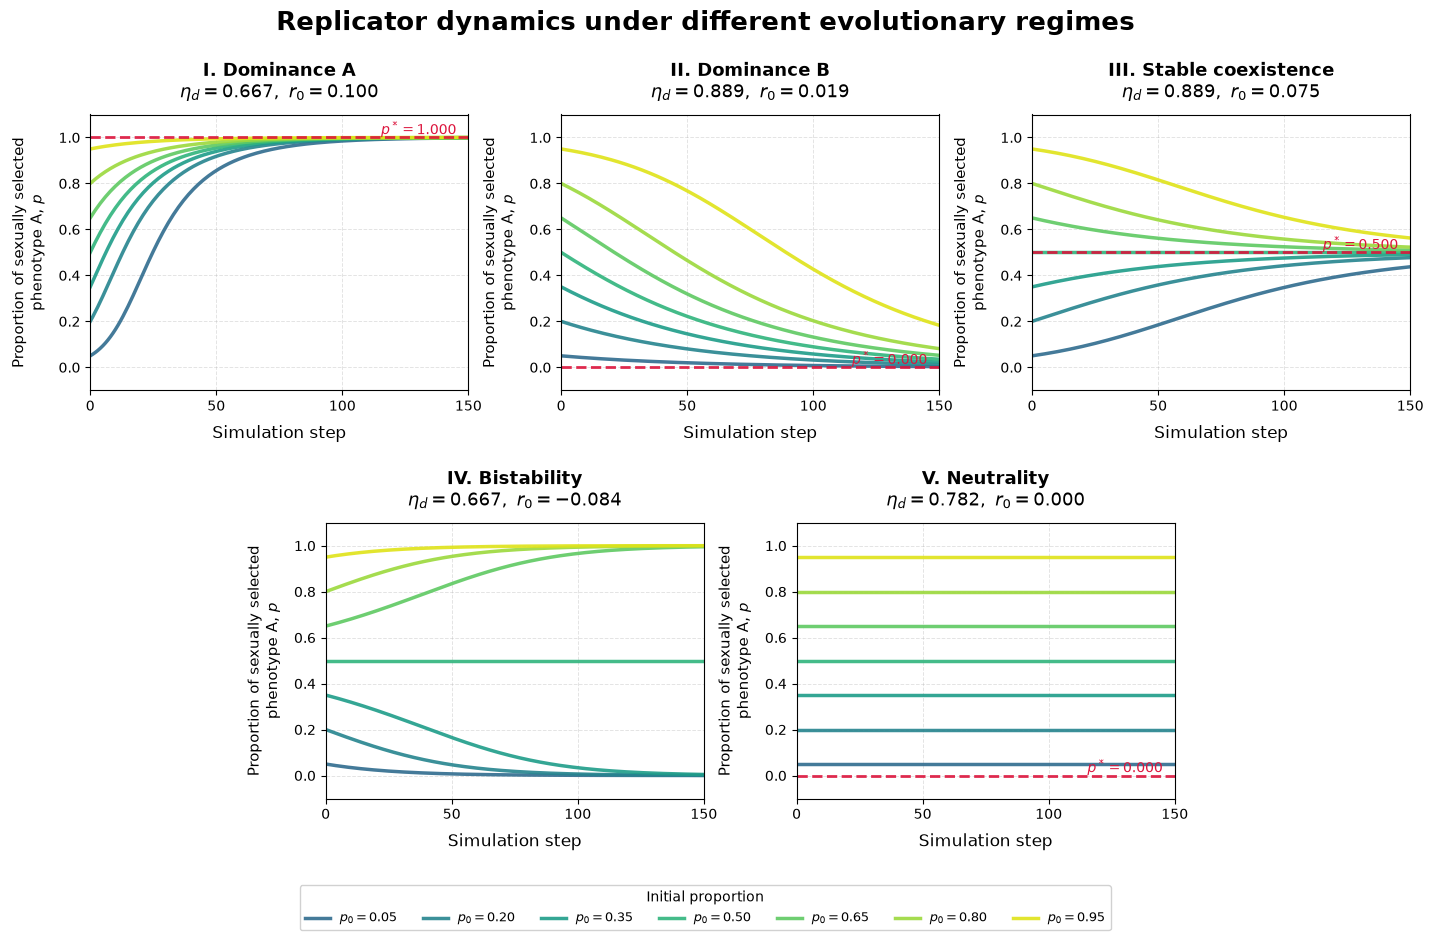
\includegraphics[width=1\linewidth]{Imagenes/Replicator.png}
    \caption{Deterministic replicator dynamics of the sexually selected phenotype A under five evolutionary regimes: (I) A dominance, (II) B dominance, (III) stable coexistence, (IV) bistability, and (V) neutrality. Each curve represents a different initial phenotype frequency ($p_0$), while predation intensity ($\eta_d$) and reproductive advantage ($r_0$) remain fixed within each scenario. The horizontal axis represents simulation steps in arbitrary time units, and the vertical axis represents the proportion of phenotype A. The corresponding frequencies maximizing mean population fitness are $p_{\max}\approx0.7105$, $0$, $0.25$, and $1$ for regimes I--IV, respectively. In the neutral regime (V), mean fitness is constant for all population compositions. These fitness maxima do not necessarily coincide with the stable evolutionary equilibria.}
    \label{fig:replicator}
\end{figure}



\begin{table}[!ht]
\centering
\caption{Evolutionary regimes obtained from the numerical
parameter search of the constant-payoff model. The parameters
$\eta_d$ and $r_0$ were determined using SciPy. A dominance,
B dominance, stable coexistence, and neutrality were identified,
whereas bistability was not found within the investigated
parameter range.}
\label{tab:linermatrixdynamics}

\begin{tabular}{l c c l c}
\toprule
Regime & $\eta_d$ & $r_0$ &
Equilibrium / stability & ESS \\
\midrule

A dominance
& $0.593052$ & $0.082638$
& $p^*=1$ (stable) & A \\

B dominance
& $0.937813$ & $0.026465$
& $p^*=0$ (stable) & B \\

Stable coexistence
& $0.870670$ & $0.244946$
& $p^*=0.873261$ (stable) & Mixed \\

Neutrality
& $0.781889$ & $\approx 0$
& All $p$ (neutral) & None \\

\bottomrule
\end{tabular}
\end{table}




\subsection{Frequency-Dependt  Evolutionary Equilibria}

We computationally analyzed the frequency-dependent replicator equation by sweeping predation intensity (\(\eta_d\)) and the initial proportion of phenotype A (\(p_0\)). This parameter sweep revealed two evolutionary regimes (table \ref{tab:frequencydependentdynamics}): A dominance and stable A-B coexistence. The figure \ref{fig:replicator} displays the deterministic trajectories for \(\eta_d = 0\) and \(\eta_d = 0.510\) across seven initial population compositions. Although the convergence paths differ, trajectories converge to the same equilibrium for a given \(\eta_d\), regardless of \(p_0\). However, this equilibrium frequency shifts with \(\eta_d\) (see \texttt{tabla\_dinamicas\_frecuencia.csv} in the notebook). We excluded the boundary conditions \(p=0\) and \(p=1\) (pure populations of B or A, respectively) because they are stationary states of the replicator equation (\(\dot{p}=0\)). Consequently, only initial proportions \(0 < p_0 < 1\) were plotted to illustrate convergence toward the evolutionary equilibria.\\ 


\begin{figure}[h!]
    \centering
    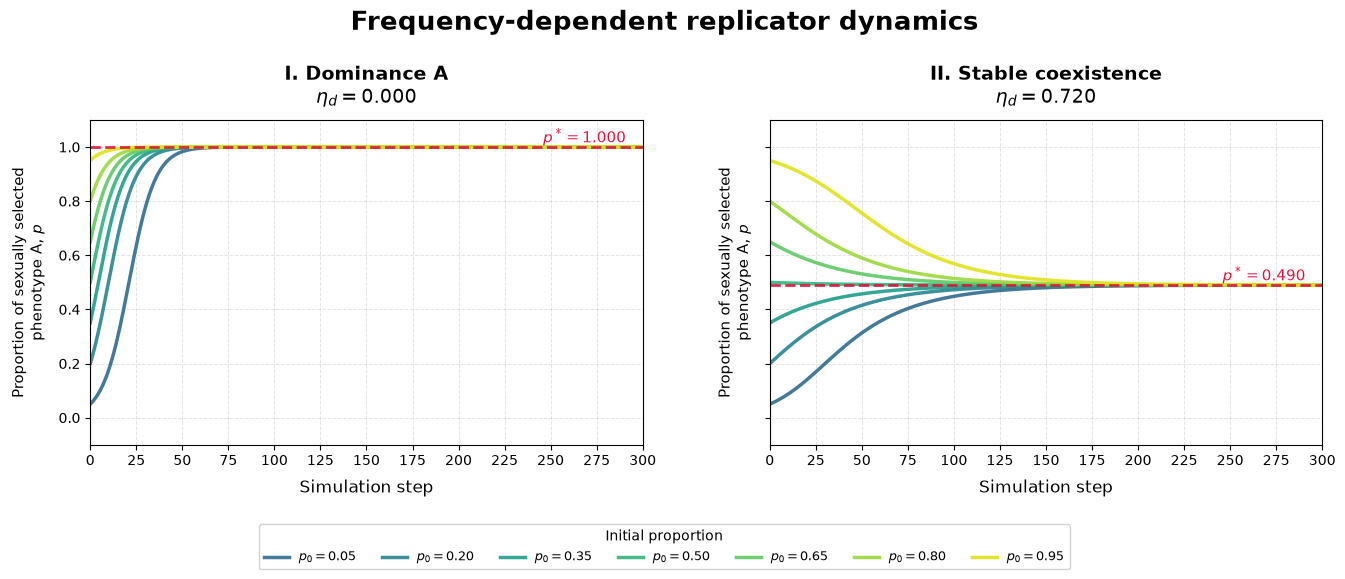
\includegraphics[width=1\linewidth]{Imagenes/ReplicatorFreqDep.png}
    \caption{ Deterministic replicator dynamics of the sexually selected phenotype A under two evolutionary regimes: (I) dominance of phenotype A at \((\eta_d=0)\) and (II) stable coexistence at \((\eta_d=1)\). Each curve represents a different initial proportion of phenotype A (\(p_0)\), while predation intensity \(\eta_d)\) remains fixed within each scenario. The horizontal axis represents simulation steps in arbitrary time units, whereas the vertical axis represents the proportion of phenotype A in the population, \(p\). In both regimes, trajectories with different initial proportions converge toward the same equilibrium, determined by the corresponding predation intensity.}
    \label{fig:replicatorFreqDep}
\end{figure}


\begin{table}[!ht]
\centering
\caption{Summary of the evolutionary regimes observed
in the frequency-dependent payoff model as a function
of predation intensity ($\eta_d$). The transition
between dominance of phenotype A and stable coexistence
occurs at approximately $\eta_d = 0.510$.}
\label{tab:frequencydependentdynamics}

\begin{tabular}{l c l c}
\toprule
Regime & $\eta_d$ & Stable equilibrium & ESS of A \\
\midrule
A dominance
& $0 \leq \eta_d < 0.510$
& $p^*=1$ & Yes \\

Stable coexistence
& $0.510 < \eta_d \leq 1$
& $0<p^*<1$ & No \\
\bottomrule
\end{tabular}
\end{table}

\clearpage 

\subsection{Stochastic Dynamics and Fixation}

\subsection{Effects of Nonlinear Sexual Saturation}

\subsection{Comparasion of Evolutionary Models}


\section{Discussion}

Porta eget eu magnis luctus vestibulum ad interdum litora platea neque sed at felis urna velit, a fusce laoreet aptent sapien fringilla montes posuere facilisi iaculis orci libero penatibus nullam. Montes scelerisque quisque phasellus praesent per sed iaculis, porttitor proin penatibus varius luctus cras primis cubilia, fusce rhoncus vestibulum magnis vitae tincidunt. Dignissim mollis lacus pharetra semper lobortis id convallis natoque porta orci, magnis venenatis sodales erat metus integer vitae habitasse conubia, congue est enim dis interdum quisque egestas sociosqu aenean. \\ 





Primero, la dependencia de la frecuencia. Compararías si introducir una vulnerabilidad que cambia con la composición del cardumen modifica las condiciones de coexistencia respecto al modelo de pagos constantes. Aquí puedes hablar de los mecanismos biológicos, incluidos oddity y confusion, sin afirmar que tus funciones representan exactamente todos esos efectos.\\ 

Segundo, la diferencia entre coexistencia determinista y persistencia estocástica. Esta sería posiblemente la comparación más potente desde la física estadística: la existencia de un equilibrio estable no garantiza la permanencia de ambos fenotipos en una población finita sin mutaciones.

Tercero, la saturación sexual. Discutirías si una ventaja reproductiva que disminuye con la abundancia de machos atractivos puede contrarrestar o reforzar los efectos de la depredación. Aquí sería importante aclarar qué parte de esa función es una hipótesis fenomenológica y qué parte está motivada por evidencia biológica. 

\subsection{Linear Payoff Matrix }
The constant-payoff model provides a deterministic reference for examining the competition between sexual selection and predation. As shown in table \ref{tab:linermatrixdynamics} and figure \ref{fig:replicator}, three main evolutionary regimes emerge: dominance of phenotype A, dominance of phenotype B, and stable coexistence. Phenotype A is favored at lower predation intensities, whereas stronger predation may favor phenotype B unless the reproductive advantage \(r_0\) is sufficient to maintain an interior equilibrium. Two additional cases were examined: bistability, in which the evolutionary outcome depends on the initial population composition, and neutrality, where the fitness difference vanishes and all population compositions remain stationary. However, bistability requires \(r_0<0\), representing a reproductive disadvantage for phenotype A and therefore falling outside the biologically motivated parameter range. It is consequently retained as a mathematical extension, while neutrality represents a limiting case in which neither phenotype has a selective advantage. \\ 



 *Se incluyó inicilamente el metodo Wright- Fisher como un método de comparación. Se vio muy claramente que no era muy realista y que no se ajustaba a la realidad de la población de peces guppy. Por lo tanto, se decidió no incluirlo en el análisis final.\\

\section{Conclusion}

Ola por temrinar


\subsection{Future Work}

Modeling poblational dynamic for depreators, instead of assuming a constant density, would allow for a more realistic relationship and observe oscillations like those of the Lotka-Volterra model . It is also interesting to analyze under Kolmogorov's theorem, which allows saturating and modulating the growth of prey and predators to obtain oscillations without losing realism, as discussed in chapter 4 of Nowak and in chapter 6 of Brauer\cite{nowakEvolutionaryDynamicsExploring2006, brauerMathematicalModelsPopulation2012}. It would also be valuable to incorporate evolutionary game theory on graphs or spatially structured games (chapters 8 and 9 of Nowak), to better understand why animals like guppies form shoals under predation and how they behave within the group; although cellular automata-type simulation could be costly due to its execution time, kaleidoscopic graphs like those proposed by Nowak remain a potentially useful tool for understanding how the fitness landscape is influenced \cite{nowakEvolutionaryDynamicsExploring2006}. For this aport could be useful the thesis of Seghers to understand the behaviour of guppies according the space \cite{hendrikANALYSISGEOGRAPHICVARIATION, reznickExperimentalStudiesEvolution2019}. \\
\clearpage
% ---------- Agradecimientos ----------
% =============================================================
% AGRADECIMIENTOS
% El uso de \section*{\centering ...} reproduce exactamente el tamaño,
% peso, posición y espaciado del encabezado del PDF de referencia.
% =============================================================
\thispagestyle{empty}
\section*{\centering Acknowledgements}

I extend my appreciation to Universidad de los Andes for providing access to excellent classes, instructors and colleagues. I would like to express my sincere gratitude to my mentors, Juan Manuel and Eli, who gave me the freedom to imagine, think outside the box and to strengthen my physical intuition. Finally, i would also like to acknowledge
the previous work of researchers such as Olga González, 
whose thesis on evolutionary game theory 
\cite{lopezRelevanciaModeloPiedra2024} was valuable 
to my own research. \\ 

\clearpage

\clearpage 

\section{Appendix}



\subsection*{Appendix A: Examples of Sexual Signals and Predation Risk}

\begin{table}[h]
\centering
\begin{tabular}{lllll}
\textbf{Signal} & \textbf{Prey} & \textbf{Sex} & \textbf{Predator} \\ \hline \hline
\multirow{5}{*}{Acoustic} 
  & &  & Bat, \textit{Trachops cirrhosus} \\
  & &  & Opossum, \textit{Philander opossum}  \\
  & Frog, \textit{Physalaemus pustulosus}  & M & Bull frog, \textit{Leptodactylus pentadactylus} \\
  &  & & Crab, \textit{Potamosarcinus richmondi}  \\
  & Cricket, \textit{Gryllodes integer} & F & Gecko, \textit{Hemidactylus tursicus} \\ \hline
\multirow{3}{*}{Visual} 
  & Guppy, \textit{Poecilia reticulata} & M & Various piscivores, e.g. Cichlidae.\\
  &&&Cyprinodontidae \\
  & Firefly, \textit{Photinus collustrans} & F & Spiders, Lycosidae  \\
  & Fireflies, e.g. \textit{Photinus} spp. & M & Fireflies (F), \textit{Photuris} spp. \\ \hline
\multirow{2}{*}{Olfactory} 
  & Mouse, \textit{Peromyscus maniculatus bairdi} & F & Weasel, \textit{Mustela nivalis} \\
  & Stink bug, \textit{Nezara viridula} & M & Tachinid fly, \textit{Trichopoda pennipes} \\ \hline
\end{tabular}
\caption{Examples of sexual signals that increase predation risk M for Males and F for Females by Magnhagen \cite{magnhagen1991}.}
\label{tab:1}
\end{table}

\subsection*{Appendix B: Code for Moran Process Simulation}
\label{app:code_moran}

The following Python 3.11.4 scripts detail the computational implementation of the Moran process and the mutation algorithms described in the Methodology. First, we define the functions for population initialization and the two mutation models:

\begin{verbatim}
def populationDef(N, p):
    """Creates a population of size N with proportion p of type A."""
    if p == 0: 
        population = ['B'] * (N - 1) + ['A']
    elif p == 1:
        population = ['A'] * (N - 1) + ['B']
    else:
        population = ['A'] * int(p * N) + ['B'] * int((1 - p) * N)
    return population

def mutacionPeriodica(generacion, intervalo, population):
    """Applies a reversible mutation every `intervalo` generations."""
    if generacion % intervalo == 0:
        idx = np.random.randint(len(population))
        population[idx] = "B" if population[idx] == "A" else "A"
    return population
    
def mutacionPoisson(population, mu):
    """Applies mutations to the population following a Poisson distribution."""
    lam = len(population) * (1 / mu)                      
    k = stats.poisson.rvs(lam)  # Actual number of mutations
    if k == 0:
        return population
        
    k = min(k, len(population))                   
    idxs = np.random.choice(len(population), size=k, replace=False)

    for idx in idxs:
        population[idx] = "B" if population[idx] == "A" else "A"
    
    return population
\end{verbatim}

Finally, the core dynamic simulation function executes the Moran process, incorporating the fitness calculations based on the sexual success and predation parameters, and applying the chosen mutation regime:

\begin{verbatim}
def MPFitDinamico(N, p, eta_d, T, g, poisson, s_a, s_b, d_a, d_b, mu):
    """
    Simulates a Moran process for a population of size N, with an initial 
    proportion p of type A individuals, over T generations.
    Returns the final proportion of A, the history, and the fitnesses.
    """
    population = populationDef(N, p)
    history = []
    p0 = p 
    
    # Initial fitness calculations
    fit_a = (1 + s_a * (1 - eta_d)) / (1 + d_a * eta_d * p0)
    fit_b = (1 + s_b * (1 - eta_d)) / (1 + d_b * eta_d * (1 - p0))

    for t in range(T):
        # Reproduction: choose based on fitness weights
        reproducer = random.choices(
            population,
            weights=[fit_a if x == 'A' else fit_b for x in population]
        )[0]
        
        # Death: choose randomly
        to_die = random.choices(population)[0]
        
        # Replace the dead individual with the offspring
        population[population.index(to_die)] = reproducer 
        
        # Apply mutations if applicable
        if g > 1:  # Periodic mutation
            population = mutacionPeriodica(t, g, population)
        elif poisson: # Poisson mutation
            population = mutacionPoisson(population, mu)
            
        # Update frequency of A and record history
        p0 = population.count('A') / len(population)
        history.append(p0)
        
        # Update fitnesses for the next generation
        fit_a = (1 + s_a * (1 - eta_d)) / (1 + d_a * eta_d * p0)
        fit_b = (1 + s_b * (1 - eta_d)) / (1 + d_b * eta_d * (1 - p0))

    return round(population.count('A') / len(population), 1), history, fit_a, fit_b
\end{verbatim}

\subsection*{Appendix C: Calculation of biological parameters}
\label{sec: Appendix Sa, Sb, Da, Db, mutation}

\subsubsection*{Relative Sexual Success and Predation Parameters}

The sexual success parameters \((S_a=0.86)\) and \((S_b=0.53)\) were estimated from the experimental observations reported by Houde \cite{houdeMATECHOICEBASED1987}\footnote{In Houde's experiments, females were presented with males from four different orangeness classes (A: most orange, to D: least orange). The time to mating (from the first display to copulation) was recorded and ranked within each trial (1 = fastest, 4 = slowest). The average relative sexual success was then calculated for the most attractive (A) and least attractive (D) phenotypes, which are fully compiled in Table 1 of \cite{houdeMATECHOICEBASED1987}. This yields \(D_a = 0.86\) for class A and \(S_b = 0.53\) for class D.}. Specifically, the relative mating performance of the most conspicuous (class A) and least conspicuous (class D) males was quantified using their mating-time rankings across ten experimental trials. These rankings were converted into normalized relative scores according to equation \ref{eq:S}. \\ 

\begin{equation}
    S=\frac{1}{10}\sum_{i=1}^{10}\frac{5-R_i}{4}
    \label{eq:S}
\end{equation}


where \((R_i)\) represents the mating-time rank in trial \((i)\), with lower ranks corresponding to faster mating. The resulting values were interpreted as relative reproductive-success indices rather than directly measured mating probabilities. For modeling purposes, these normalized scores were assigned probability-like weights within the fitness functions, providing a phenomenological representation of the reproductive advantage associated with each phenotype.\\ 

Similarly, the predation parameters \((D_a=0.107)\) and \((D_b=0.023)\) were estimated from the predator-preference experiments conducted by Godin and McDonough \cite{godinPredatorPreferenceBrightly2003}  \footnote{In the experiments of Godin and McDonough, the cichlid predators attacked the brightly colored males first in approximately \(80\%\) of the trials, whereas they attacked the drab males first in approximately \(20\%\). Once an attack was initiated, the conditional probability of capture was calculated as the number of males captured divided by the total number of males attacked. For the brightly colored males, this probability was \(0.137\), while for the drab males it was \(0.103\). Multiplying these respective probabilities yields the parameters \(D_a\) and \(D_b\).}. These values were obtained by combining the probability of being attacked first with the conditional probability of capture following that initial attack using equation \ref{eq:D}. \\ 

\begin{equation}
    P(\text{initial attack and capture})=
P(\text{attacked first})
P(\text{captured}\mid\text{attacked first}).
    \label{eq:D}
\end{equation}


The resulting quantities represent relative indices of vulnerability under the experimental conditions, rather than universal probabilities of mortality in natural populations. Accordingly, they were incorporated into the fitness functions as probability-like weights to represent differences in predation costs between conspicuous and less conspicuous male guppies. This approach preserves the relative effects reported experimentally while providing dimensionless parameters suitable for the evolutionary model. \\ 



\subsubsection*{Mutation}

Two alternative mutation mechanisms were considered to introduce stochastic transitions between the modeled phenotypes a \textbf{periodic mutation scheme} and a \textbf{Poisson-based mutation process}. \\ 

In the periodic scheme, one individual is randomly selected to undergo a reversible transition between phenotypes A and B after a prescribed number of simulation iterations. In the Poisson scheme, the number of mutation events is sampled from a Poisson distribution,

\begin{equation}
    P(K=k)=\frac{e^{-\lambda}\lambda^k}{k!},
    \label{eq:poisson}
\end{equation}

where $\lambda$ represents the expected number of mutation events over the specified time interval. \\ 

To establish a biologically motivated reference timescale, the average germline mutation rate reported for fishes by Bergeron et al. \cite{bergeronEvolutionGermlineMutation2023} was adopted:

\begin{equation}
    \mu_{\mathrm{site}}
    =5.97\times10^{-9}
    \ \text{mutations per site per generation}.
\end{equation}

Kottler et al. \cite{kottlerAdenylateCyclase52015} identified a genomic region of approximately $L=118\,000$ base pairs associated with the \textit{blond} pigmentation phenotype in guppies, containing the \textit{adcy5} gene. Assuming a uniform mutation rate across this region, the expected number of mutations per genomic-region copy per generation was approximated as

\begin{equation}
\begin{aligned}
    u &= \mu_{\mathrm{site}}L\\
      &= (5.97\times10^{-9})(118\,000)\\
      &\approx 7.04\times10^{-4}.
\end{aligned}
\label{eq:regional_mutation_rate}
\end{equation}

Since this value is small, the reciprocal provides an approximation to the mean waiting time for a mutation within one copy of the considered genomic region:

\begin{equation}
    \mu^*=\frac{1}{u}
    \approx 1.42\times10^3
    \ \text{generations}.
    \label{eq:mutation}
\end{equation}

For a population containing $N$ individuals, the Poisson model assumes one effective copy of the considered region per individual and independent mutation events. Under these assumptions, the expected number of regional mutations per generation is

\begin{equation}
    \lambda_{\mathrm{gen}}
    =Nu
    =\frac{N}{\mu^*}.
    \label{eq:poisson_parameter}
\end{equation}

Accordingly, the corresponding population-level mean waiting time between mutation events is approximately $\mu^*/N$ generations, rather than $\mu^*$.  The periodic and Poisson schemes therefore represent different temporal distributions of mutation events. To compare them at equivalent average mutation frequencies, the interval between periodic events must be chosen consistently with the expected population-level mutation rate. \\ 

In the computational simulations, mutation events were applied as reversible transitions between phenotypes A and B. These transitions provide a simplified representation of genetic variation and do not explicitly resolve the underlying molecular mechanisms. \\ 

Importantly, mutations within the considered genomic region do not necessarily produce observable changes between the two modeled phenotypes. Consequently, the estimated mutation timescale should not be interpreted as a directly measured phenotype-switching rate. Values on the order of $10^3$--$10^4$ generations provide an exploratory range for examining the sensitivity of the models to mutation frequency. \\ 

Furthermore, the biological mutation estimates are expressed per generation, whereas the Moran process advances through individual reproduction--replacement events. A conversion between these timescales is required for a quantitatively calibrated mutation process. The mutation mechanisms implemented here are therefore treated as exploratory extensions rather than direct predictions of mutation occurrence in natural guppy populations.



%---Firma Directa ---
\begin{figure}[h!]
    \centering
    
\includegraphics[width=0.45\linewidth]{Imagenes/firmadirector.png}\\

\end{figure}

% ---------- Referencias ----------
\clearpage
\printbibliography[heading=bibintoc, title={References}]
\end{document}
